
\section{Background}\label{sec:bg_stability}


\begin{center}
\begin{table}
\begin{tabular}{l|l|p{3.15in}} 
{\bf Year} & {\bf Author} & {\bf Major Results} \\ \hline 
1996 & Varadhan \ea~\cite{Varadhan1996,Varadhan2000} & Observed that
policy-based 
routing protocols may never converge (\ie, they may be ``unsafe''). \\
%
1999 & Griffin \ea~\cite{Griffin2002c,Griffin99} & Showed NP-hardness of
determining safety, and derived sufficient global conditions for
safety. \\ 
%
2001 & Gao and Rexford~\cite{Gao2001a} & Derived restrictions
on routing configuration and topology that guarantee safety, and
observed that these conditions are similar to common practice. \\ 
%
2003 & Sobrinho~\cite{Sobrinho2003} & Developed an algebraic framework
for general path vector, policy-based protocols and derived properties
that the algebra must have to guarantee convergence. \\
%
2003 & Griffin
\ea~\cite{Griffin2003} & Laid out design tradeoffs in policy-based
routing protocols: expressiveness, modularity, etc.\\ 
%
2004 & Jaggard and Ramachandran~\cite{Jaggard2004} & Designed tests for
dispute wheels. \\ 
%
2005 & Griffin and Sobrinho~\cite{Griffin2005} & Developed a framework
called ``metarouting'', useful for constructing routing protocols that
are guaranteed to converge. 
\end{tabular}
\caption[Results from previous work on global routing
stability.]{Results from previous work on global routing
stability. 
Chapter~\ref{chap:policy} builds on many of these results.} 
\label{tab:stability_results}
\end{table}
\end{center}


Because Internet routing is policy-based, and each AS has the
flexibility to define its own policies independently of other ASes, the
policies of one AS may interact with those of another to cause the
protocol to oscillate.  Table~\ref{tab:stability_results} surveys
previous and ongoing work in this area.

A seminal paper by Varadhan \ea observed that policy-based interdomain
routing protocols could oscillate and defined the concept of {\em
safety}~\cite{Varadhan1996,Varadhan2000}.  Varadhan
\ea also conjectured that routing systems that allow rankings other than
those based on next-hop rankings or shortest path routing may be
unsafe~\cite{Varadhan1996,Varadhan2000}.  In fact, in
Section~\ref{sec:nexthop}, we show that even routing systems that only
allow next-hop rankings are not safe.


Griffin \ea asked how expressive an autonomous, robust routing system
can be~\cite{Griffin2003}; we address this
question in this chapter.  Varadhan
\ea showed that a routing system with an acyclic topology will have at
least one stable path assignment if participants can only express
next-hop preferences~\cite{Varadhan1996,Varadhan2000}.  We show
that when BGP's protocol dynamics are taken into account, restricting
each AS to only next-hop rankings does {\em not} guarantee that the
routing system will be safe (even though the routing system always has
at least one stable path assignment).


Gao and Rexford derived sufficient constraints on rankings, filtering,
and network topology
to guarantee routing stability; they also observe that these
constraints reflect today's common practice~\cite{Gao2001b,Gao2001a}.
%Gao and Rexford state sufficient conditions for safety in eBGP and
%observe that typical policy configurations satisfy these
%conditions~\cite{Gao2001a}.  
They showed that if every AS considers each of its neighbors as either a
customer, a provider, or a peer, and obeys certain local constraints on
rankings and filtering, and if the routing system satisfies certain
topological constraints, then BGP is stable.\footnote{Griffin {\em et al.}
noted that analogous sufficient conditions apply to iBGP with route
reflection~\cite{Griffin2002}, although we show in
Chapter~\ref{chap:rlogic} that these conditions are unnecessarily
strong.}  However, their model does not incorporate ranking
autonomy, because their proposed topological constraints are global.

Griffin's sufficient conditions require global knowledge of rankings;
those of Gao and Rexford require global knowledge of the AS-level
topology. Our goal is to derive constraints that must hold on the
configuration of a single AS {\em without any global knowledge}.
%Our recent work derived necessary conditions that the
%configuration of each AS must satisfy to guarantee
%safety~\cite{Feamster2005}.
%
Furthermore, Griffin's work does not consider the effects of filtering;
the conditions of Gao and Rexford restrict quite severely. The example below
illustrates why these restrictions may sometimes be too strict.  


%%%%%%%%%%%%%%%%%%%%%%%%%%%%%%%%%%%%%%%%%%%%%%%%%%%%%%%%%%%%
% EXAMPLE

\begin{figure}
\centering
\begin{psfrags}
%
\psfrag{d_1}{{\Large $d_1$}}
\psfrag{d_2}{{\Large $d_2$}}
\psfrag{d_3}{{\Large $d_3$}}
%
\resizebox{0.8\columnwidth}{!}{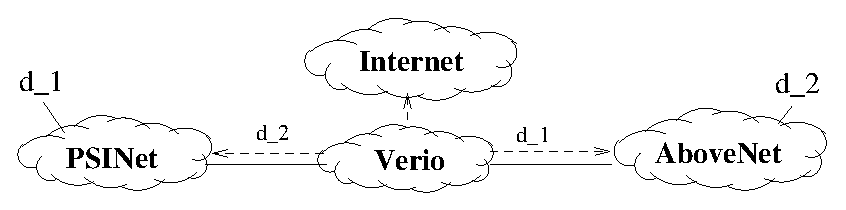
\includegraphics{figures/depeer.eps}}
%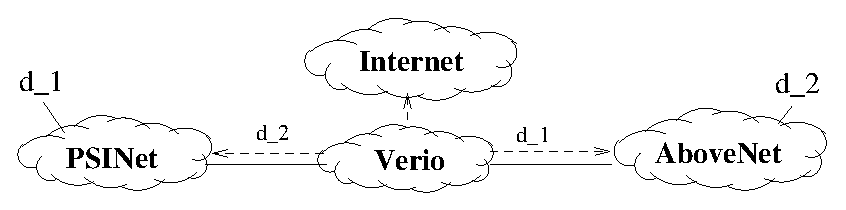
\epsfig{file=figures/depeer.eps,width=0.45\textwidth,height=0.9in}
\end{psfrags}
\caption{Constraints on filtering and topology are not enforceable. }
\label{fig:depeer}
\end{figure}

\begin{example}
\label{ex:depeer}
Figure~\ref{fig:depeer} shows a situation that occurred 
in 2001~\cite{bush:privcomm}.  When PSINet terminated
its peering with AboveNet, AboveNet lost connectivity to
PSINet's customers, $d_1$.  To restore connectivity, AboveNet
bought ``transit'' service from Verio (already a peer of PSINet), but
only for routes to PSINet and its customers.
%\footnote{Thanks to
%Randy Bush for this anecdote.}

%Verio treats AboveNet as a customer, advertising $d_1$ (and all of
%PSINet's prefixes) to AboveNet.  
Verio does not filter $d_1$ (or any of PSINet's prefixes) from AboveNet,
which is only possible if Verio treats AboveNet as a customer.
The constraints imposed by Gao and
Rexford state that an AS {\em must} prefer customer routes over peering
routes.\footnote{Gao and Rexford present a weaker constraint that allows
an AS to rank routes learned from customers and peers over those from
providers, but does {\em not} require customer routes to be strictly
preferred over routes from peers.  This relaxed condition requires that
there are no instances where an AS's customer is also a peer of another
one of the AS's peers.  Of course, the example shown in
Figure~\ref{fig:depeer} could also 
violate this 
constraint on the topology: PSINet is Verio's customer for $d_1$, but it
would be reasonable for PSINet to peer with another of Verio's peers,
since all are ``tier-1'' ISPs.}  
%
%The first constraint requires Verio to export a route to $d_3$ to the
%rest of the Internet (hence, requiring it to carry traffic to AboveNet's
%destination $d_3$ from {\em any} other network, not just
%PSINet).
%
This constraint requires Verio to rank AboveNet's route to $d_2$ over
any other available routes to $d_2$ in order to guarantee stability,
which restricts Verio's flexibility in how it can select
routes.
Establishing a new business
relationship (and, hence, altering its filtering policies) {\em requires} Verio
to change its rankings as well.
%
\end{example}



The framework of Gao and Rexford is also too strict because it assumes
that a pair of ASes has only a single type of business relationship. For
multinational ISPs, this assumption is constantly violated: two ASes may
have a peering relationship over sessions in one geographic region, but
one may purchase transit from the other in another geographic region.

\begin{figure}
\centering
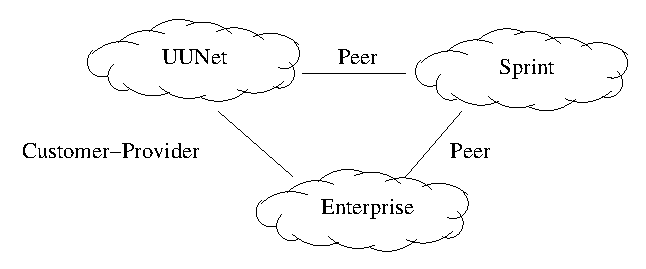
\epsfig{file=figures/peerprov.eps, width=0.8\linewidth}
\caption[Pairs of ASes may have different relationships
in different geographic regions.]{Pairs of ASes may have different
business relationships 
in different geographic regions.}
\label{fig:peerprov}
\end{figure}


\begin{example}
Consider Figure~\ref{fig:peerprov}; there are hundreds of similar
real-world examples~\cite{bush:privcomm}.  AS~1 and AS~2, two ISPs, peer
in North America, but AS~1 buys service from AS~2 in Europe (in
practice, this arrangement may occur if AS $1$ does not have a European
backbone).  AS~1 will typically learn {\em all} destinations (\ie,
European and North American) over its customer link, but just the North
American destinations over its peering link.  Suppose that AS~2 peers
with AS~3 in North America, and AS~1 peers with AS~3 in Europe.  The
router in AS~2 that has a peering relationship with AS~3 will advertise
the European routes from its customer link; AS~3 also learns those via
its peering session with AS~1.  This arrangement is precisely the
``peer-provider'' cycle that is prohibited some of the convergence
conditions of Gao and Rexford (\eg, Guideline A,~\cite{Gao2001a}).  This
scenario mandates that AS~2 prefer the route to the destination via
AS~1, rather than another peer through which it may have a route to the
same destination.
\end{example}


%% \noindent
%% This example demonstrates that the conditions suggested by Gao and Rexford
%% may be too strong to enable ASes to implement flexible
%% contracts.
%% %: according to these conditions, providing a
%% %service to AboveNet requires Verio to restrict both its ranking and its
%% %filtering.  
%% Hence, we are motivated to
%% study stability conditions for routing protocols, assuming that ASes are
%% completely 
%% unrestricted in how they filter.


Various previous work has studied {\em global} conditions to guarantee
the safety of routing systems; global conditions presume that the
routing system does not preserve local choice of rankings (\ie, ranking
autonomy).  Griffin \ea showed that, if the rankings of the ASes in
a routing system do not form a \emph{dispute wheel} (a concept that
describes global relationship between the rankings of a set of ASes),
then the routing system is safe~\cite{Griffin2002c}.  Griffin \ea also
examined {\em robustness}, the property that safety is guaranteed even
if arbitrary nodes or edges are removed from the graph.  We view
robustness as a special case of filtering: removing an edge can be
achieved if the ASes incident to that edge filter all routes through
that edge; removing a node entails having all ASes filter all routes
through that node.

%  Note that a dispute wheel
%does not fully characterize routing instability, because there are safe
%routing systems that have dispute wheels.  This paper presents a special
%case of a dispute wheel, called a dispute ring, and proves that a
%routing system with a dispute ring is unsafe under arbitrary filtering.
Griffin \ea also showed how to modify a BGP-like path vector protocol to
detect the existence of a dispute wheel but left unspecified how the
ASes should resolve the dispute wheel~\cite{Griffin2000}.  Machiraju and
Katz defined a new global invariant for determining safety when at most
one AS deviates from the conditions of Gao and
Rexford~\cite{Machiraju2004}.  Govindan \ea proposed a routing
architecture where ASes coordinate their policies~\cite{Govindan1999,
Govindan1998} using a standardized policy specification
language~\cite{rfc2622}.  Jaggard and Ramachandran presented
global conditions that guarantee safety of routing systems that allow
ASes to express only next-hop preferences over routes, and designed
centralized and distributed algorithms to check these global
conditions~\cite{Jaggard2004}.  

More recent work has attempted to design policy-based protocols that are
guaranteed to converge without imposing any global conditions.  Sobrinho
defined new concepts that describe global relationships between
preferences and incorporate several previous results (including those
of both Griffin \eans~\cite{Griffin2002c} and Gao and
Rexford~\cite{Gao2001a}) into a single algebraic
framework~\cite{Sobrinho2003}.  He examined requirements for
convergence and asserted that any vectoring protocol that preserves a
property called ``strict monotonicity'' is guaranteed to converge.
Recent work on ``metarouting'' exploits this algebraic framework to
allow protocol designers to specify new routing protocols that are
guaranteed to converge by requiring algebras that preserve strict
monotonicity~\cite{Griffin2005}.  In this chapter, we will
see that the set of routing protocols that are guaranteed to converge is
apparently not much more permissive than shortest path routing, if ASes
have complete liberty in setting filters.  Metarouting may allow the
protocol designer to better explore the tradeoffs between filtering
expressiveness, ranking expressiveness, and safety (\ie, compromising
filtering expressiveness to allow for more expressive rankings).

In contrast to these studies of global conditions for safety, we study
the conditions under which a policy-based interdomain routing protocol
can be safe if it preserves the autonomy of each AS.  Our results
suggest that, allowing for complete autonomy and filtering
expressiveness, guaranteeing safety requires restricting ranking
independence essentially to preferences based on consistent weightings
of the edges in the graph.

Gouda and Schneider study classes of routing protocol metrics for which
each node in a routing tree has its most preferred path, but do not
address routing stability~\cite{Gouda2003}.

%In constrast, we explore the necessary
%and sufficient conditions to guarantee stability while imposing only
%{\em local} constraints on an AS's rankings.  The results of our work
%suggest that imposing only local constraints to guarantee stability
%may require constraints that are too strong to allow sufficiently
%expressive routing policies.  As a result, the design of new
%interdomain routing protocols may require incorporating the types of
%global checks and algorithms described in this previous work.
